The signals we obtained from the experiment were analyzed and interpreted using the methods presented in this chapter. Starting with specifics of the data collection process, we continue by discussing signal processing algorithms and feature extraction, and end with details on classification procedure.

\section{Data Collection}
As mentioned in section \ref{physmeas}, the psychophysiological measures, selected for this thesis, were blood volume pulse (\gls{bvp}), galvanic skin response (\gls{gsr}), and skin temperature. These signals were recorded using the integrated Photoplethysmography (\gls{ppg}), Electrodermal Activity (EDA), and Infrared Thermopile sensors of the Empatica E4 wristband. All recordings were conducted using a sampling frequency of 64Hz for \gls{bvp}, and 4Hz for both \gls{gsr}, and skin temperature. 
From the 14 subjects that partook in our experiment we obtained 14 sets of physiological data. The data of one subject was removed due to substantial artifact contamination, resulting in a total of 13 sets of physiological data that were used in the subsequent process. Each set was comprised of roughly 80-90 minutes of recordings, which complied to approximately 326.400 samples for \gls{bvp}, and 20.400 samples for \gls{gsr}, and skin temperature. 
The collected data was continuously streamed to a TCP client, running on the nearby Processing Unit, via a Bluetooth connection and saved into csv files after every full minute of recording. The saved files contained data samples of all three data streams and were named following the pattern shown in \ref{recpattern}.
\begin{equation} \label{recpattern}
\text{recording\_yyyy-mm-dd-hh-mm-ss}
\end{equation}
Then again, each data sample was comprised of three components which identified the data stream, the sample time, and the sample value. An example of this pattern is shown in \ref{samplepattern} for a sample of the BVP signal stream. 
\begin{equation}\label{samplepattern}
\text{E4\_Bvp 1569592961,01857 25,33795}
\end{equation}

\section{Data Preparation}
As the data was saved in a number of individual csv files the goal of the initial step of data processing was dedicated to translate the data samples into a usable format and separate the individual data stream (i.e. BVP, GSR, and skin temperature). This goal was achieved using two simple python scripts. The first program would locate all csv files in a certain folder and seamlessly merge them to a single csv file. Afterwards, the second script was used to scan all entries of this new file and sort them by their stream tag, which was indicated by the first portion of each data sample (see \ref{samplepattern}), using a simple string comparison method. This process resulted in a total of 6 data files (i.e. 2 files per data stream), of which each file contained either the sample values or the sample times of a single data stream. This format made the data easily distinguishable and accessible for the final step of data preparation, which was data segmentation. We divided the data streams into segments that were associated with the individual sessions of the experiment, using automatic timestamps that were generated during the experiment. The extracted segments were then saved in individual files that were appropriately named to provide explicit information about their content to facilitate subsequent processing steps. The naming pattern is shown in \ref{segmentpattern}.
\begin{equation}\label{segmentpattern}
\text{\_DataStream\_Datatype\_SubjectID\_SessionLabel\_StartTime\_EndTime}
\end{equation}

\section{Data Analysis}
All aspects of data analysis were handled using the programming language Python in combination with the PyCharm IDE. Therefore, this section is dedicated to explaining the general strategy, as well as the scripts that were built in the process of managing data processing, and feature extraction tasks.

\subsection{BVP}
\subsubsection{Pre-Processing}
% 	- PEAK DETECTION
%		- bandpass zero phase filtering
%		- clipping
%		- squaring
%		- moving averages
%		- thresholding
%		- blocks of interest
%		- peak detection
%		- peak validation
The main objective of BVP pre-processing was the detection of AC pulses, or $\alpha$ waves, in the BVP signal. To guarantee high quality peak detection even under challenging conditions, we implemented an algorithm that was introduced by Elgendi et al. (2013) for this very reason. The peak detection algorithm is based on event-related moving averages with dynamic thresholds, and is comprised of three main stages: pre-processing (bandpass filtering and squaring), feature extraction (generating potential blocks using two moving averages), and classification (thresholding)\cite{Elgendi2013}. 

%[insert: bvp_dt.jpg, source: \cite{Elgendi2013}]
%\begin{figure}[ht]
%	\centering
%  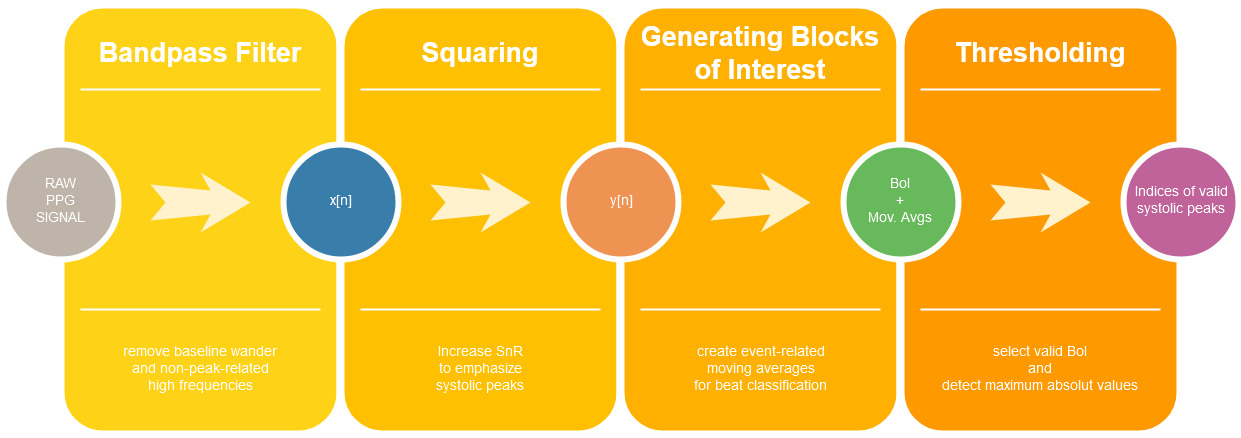
\includegraphics[width=1.0\textwidth, angle=0]{images/bvp_dt.jpg}
%	\caption[Peak Detection Algorithm]{Peak Detection Algorithm by Elgendi et al. (2013). This systolic peak time-domain detection algorithm consists of three main stages: pre-processing (bandpass filter, squaring), feature extraction (two moving averages), and classification (thresholding).}
%	\label{bvp_dt}
%\end{figure}

%The general structure of the algorithm is shown in \ref{bvp_dt}. 
The following paragraph will elaborate on the individual steps of the algorithm.\\
\textbf{Bandpass Filtering.} A zero-phase second-order Butterworth filter, with a bandpass of 0.5-8 Hz was implemented to remove baseline wander and non-peak-related high frequency components. The filter output was then applied to the raw PPG signal resulting in the filtered signal $S[n]$.\\
\textbf{Clipping.} In preparation of the next step of the algorithm, the filtered signal was clipped by removing the signal below zero. This resulted in the clipped signal $Z[n]$.\\
\textbf{Squaring.} Squaring was used to emphasize large differences resulting from the systolic waves, while simultaneously suppressing smaller differences caused by diastolic waves and noise \cite{Elgendi2013}.
This resulted in the signal $y[n]$ which is equal to $Z[n]^{2}$\\
\textbf{Generating Blocks of Interest.} Blocks of interest are generated using the two event-related moving averages $MA_{peak}$ and $MA_{beat}$. $MA_{peak}$ was used to mark systolic peak areas in $y[n]$ and is given by the equation \ref{ma_peak}. Where $W_{1}$ represented the window size of the systolic peak duration and was set to a value of 111 ms.\\
\begin{equation}\label{ma_peak}
MA_{peak}[n] = \frac{1}{W_{1}}\cdot(y[n-\frac{W_{1}-1}{2}]+...+y[n]+...+y[n+\frac{W_{1}-1}{2}])
\end{equation}
$MA_{beat}$ was used to mark heartbeat areas and given by the equation \ref{ma_beat}. Where $W_{2}$ represented the window size of one heartbeat duration and was set to a value of 667 ms.\\
\begin{equation}\label{ma_beat}
MA_{beat}[n] = \frac{1}{W_{2}}\cdot(y[n-\frac{W_{2}-1}{2}]+...+y[n]+...+y[n+\frac{W_{2}-1}{2}])
\end{equation}
\textbf{Thresholding.} The first dynamic threshold $THR_{1}$ was used to mark potential peak areas in $y[n]$ by creating a block of interest for every interval where $THR_{1}$ was greater than $MA_{peak}$. $THR_{1}$ was derived from $MA_{beat}$ following equation \ref{thr1}.
\begin{align} \label{thr1}
THR_{1} &= MA_{beat}[n]+\alpha \\
\alpha &= \beta\cdot\bar{z}
\end{align}
Where $\beta$ was set to a constant value of 0,02 and $\bar{z}$ was the statistical mean of $y[n]$. Figure \ref{bvp_dta} demonstrates the idea of using two moving averages to generate blocks of interest.\\ 
%[insert: bvp_dta.jpg, source: \cite{Elgendi2013}]
\begin{figure}[ht]
	\centering
  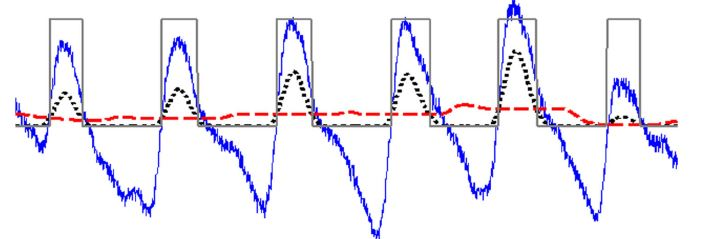
\includegraphics[width=1.0\textwidth, angle=0]{images/bvp_dta.jpg}
	\caption[Peak Detection Algorithm]{Blocks of interest are shown as grey squares over the filtered signal (in blue). The blocks are generated, using the two moving averages $MA_{peak}$ and $MA_{beat}$, which are depicted as a black dotted signal and a dashed red signal respectively. (source: doi:10.1371/journal.pone.0076585.g009)}
	\label{bvp_dta}
\end{figure}
Although this process generated many blocks, only some would contain the desired feature (i.e. the systolic peak). Therefore, it was necessary to reject the blocks that resulted from diastolic waves and noise. This rejection was based on the second threshold $THR_{2}$, which corresponded to the anticipated width of a systolic peak and was set to $W_{1}$. Whenever a block was wider than or equal to $THR_{2}$ it was classified as valid.\\
\textbf{Peak Detection.} In the last step of the algorithm systolic peaks were detected by localizing the maximum absolute value in valid blocks of interests. 

\subsubsection{Inter-Beat-Intervals}
 INTER BEAT INTERVALS
	- DETECT OUTLIER
	- DETECT ECTOPIC BEATS
	- ARTIFACT DECLARATION
	- LINEAR INTERPOLATION
\subsubsection{Data Validation}
 DATA VALIDATION
\subsubsection{Feature Extraction}
 FEATURE EXTRACTION

\subsection{GSR}
\subsubsection{Pre-Processing}
% GSR PRE PROCESSING
%	- low pass zero phase filtering
%	- smoothing: moving average filtering
\subsubsection{Feature Extraction}
% FEATURE EXTRACTION

\subsection{Skin Temperature}
\subsubsection{Pre-Processing}
% TEMPERATURE PRE PROCESSING
%	- smoothing: moving average filtering
\subsubsection{Feature Extraction}
% FEATURE EXTRACTION

\section{Data Interpretation}
% ml methods

